\section{Design Flow}
\label{sec:designflow}

\begin{figure}[ht!]
	\centering
	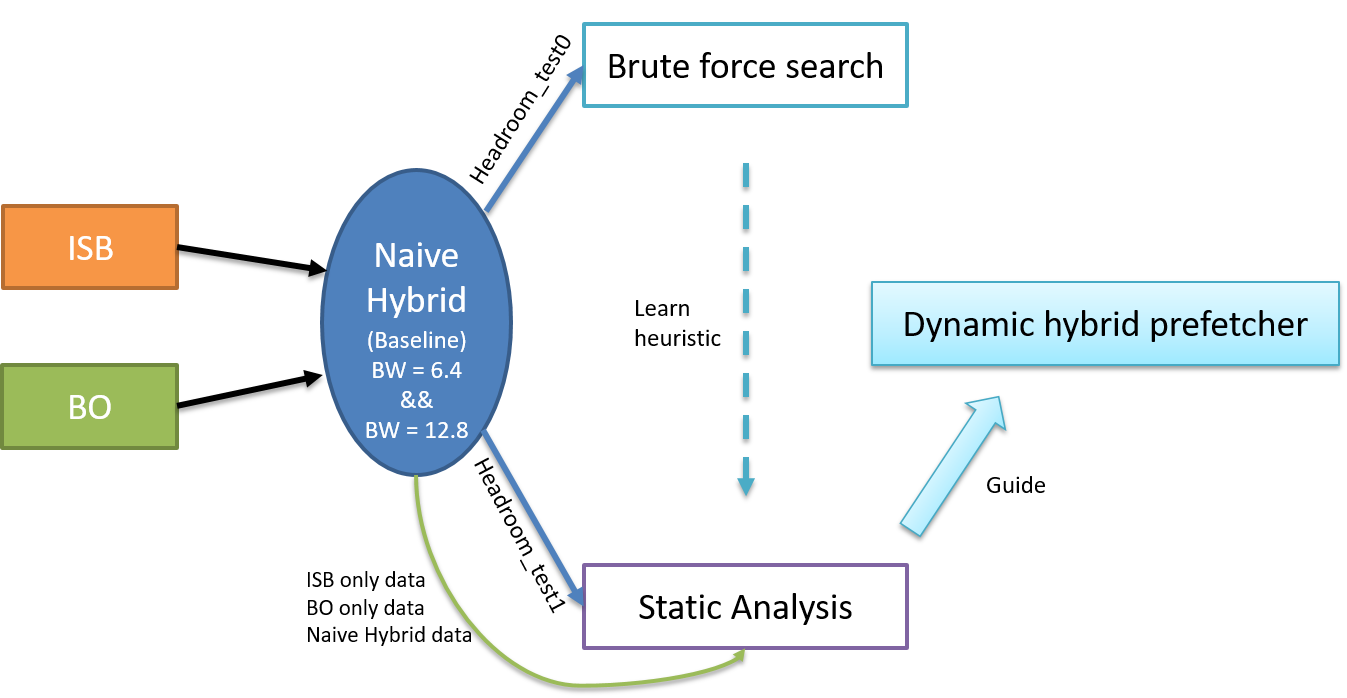
\includegraphics[width=1.0\textwidth]{images/design_flow.png}
	\caption{Design flow}
	\label{fig:design_flow}
\end{figure}

Based on the introduction and motivation we demonstrated above, we design our headroom experiments and ``smart'' hybrid prefetcher system in Fig.\ref{fig:design_flow}.

First, we will evaluate the individual performance of \emph{BO}, \emph{ISB} and \emph{NHP}. Note that here we measure performance using two different memory bandwidth configuration. 12.8 represents high memory bandwidth 12.8 GB/s and 6.4 represents low memory bandwidth 6.4 GB/s. The \emph{Brute Force Search} and \emph{Static Analysis} are both offline headroom designs which will be described in the following two sections. Briefly, \emph{Brute Force Search} tries each choice on each PC, and finds out the best decisions and optimal headroom. Static Analysis comes up with a heuristic. It uses the statistics of each PC from ISB, BO and naive hybrid experiments as input, and builds a strategy that makes decisions closest to \emph{Brute Force Search} thus achieves best speedup. Finally the Static Analysis guides the design of our final hybrid prefetch system, which will be explained in section \ref{sec:ourdesign}.

  \subsection{Brute Force Search}
  \label{sec:bruteforcesearch}

  In this part, we will first illustrate why we need a Brute Force Search to find the headroom of PC localization. Then we show how Brute Force Search headroom experiment is designed. \par

  \subsubsection{Metric to measure a PC}
  \label{sec:metricPC}

  It is known that accuracy and coverage are two good metrics \cite{yalepaper} to measure the performance of a prefetcher. They are calculated as follows:
  \begin{equation}
  Accuracy = \frac{prefetch\ hits}{total\  prefetched}
  \end{equation}
  \begin{equation}
  Coverage = \frac{prefetch\ hits}{total\ prefetch\ hits + total\ misses}
  \end{equation}

  Similarly we can define accuracy and coverage of a trigger PC:
  \begin{equation}
  PC\ Accuracy = \frac{prefetch\ hits\ by\ this\ PC}{prefetches\ by\ this\ PC}
  \end{equation}
  \begin{equation}
  PC\ Coverage = \frac{prefetch\ hits\ by\ this\ PC}{total\ prefetch\ hits + total\ misses}
 \end{equation}

 \begin{figure}[ht!]
	\centering
	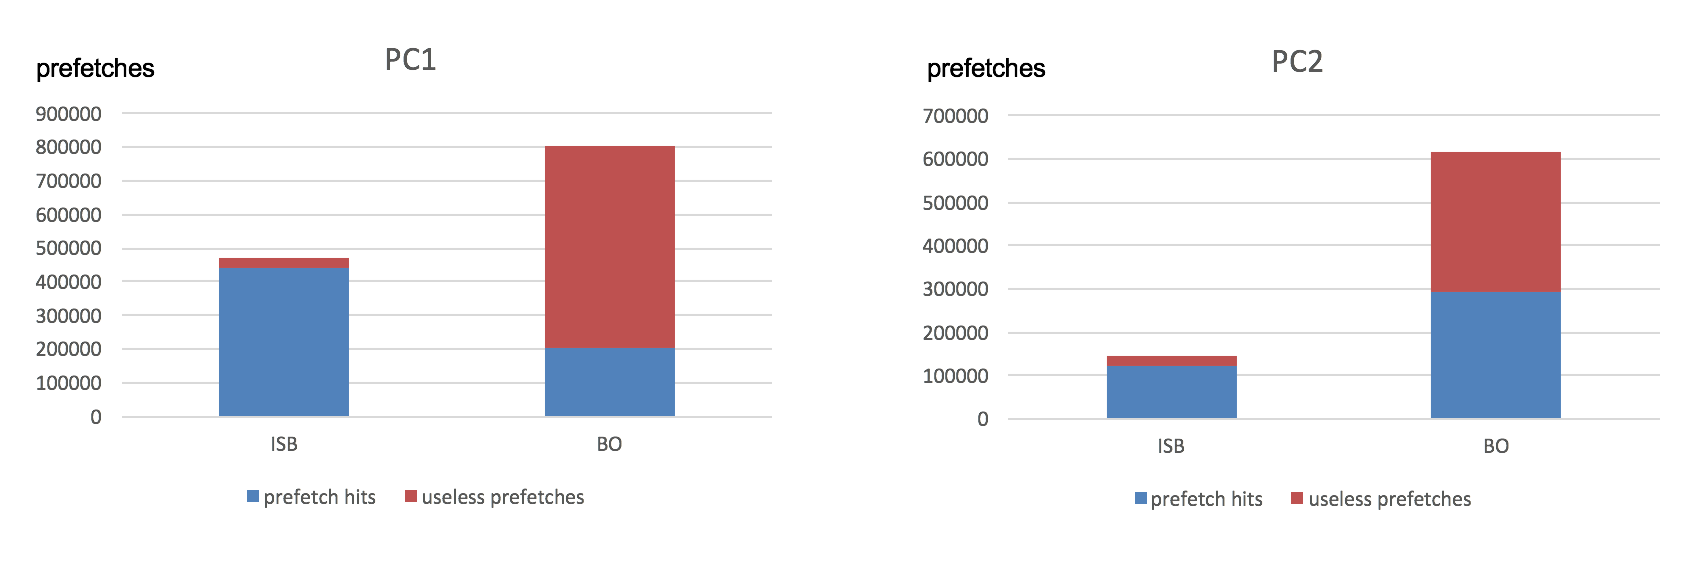
\includegraphics[width=1.0\textwidth]{images/metric.png}
	\caption{Hits and useless prefetches example}
	\label{fig:pcmetric}
\end{figure}

However, these two metrics from \emph{ISB} and \emph{BO} sometimes cannot determine the preference of a PC.
For example in Fig.\ref{fig:pcmetric}, on PC1, it is clear that ISB on this PC has higher accuracy and coverage, so the hybrid system should choose ISB. But on PC2, ISB has higher accuracy but BO has higher coverage, then it's hard to choose.
In terms of speedup, prefetch hits has positive contribution and useless prefetches has negative contribution.
On PC2, BO has more prefetch hits and more useless prefetches, so it's hard to infer its contribution is positive or negative only on this numbers.

    \subsubsection{Design of Brute Force Search}
    \label{sec:designBFS}
    Since the effect of accuracy and coverage of a PC to the overall performance is not clear, we design the Brute Force Search experiment to explore the space of PC's choices and find out the headroom. The steps are listed as follows. \par
    1) Choose several PCs with the main influence. For each pinpoint, we find out the PC with the most prefetches, denoted this number as MAX. Any PCs that has prefetches more than 5\% of MAX are chosen.\par
    2) Find the best decision for each PC. For each PC, run four experiments, respectively set its decision to ISB, BO, neither or both. \textbf{All other PCs are set to choose both}.\par
    3) Combine the best decisions of all PCs.\par
    Note that for the several PCs we consider, they can cover more than 95\% of total prefetches, so they can represent the prefetch charactaristic of a benchmark. \par
    Here the Brute Force Search design is not optimal. An optimal exploration should run all the possible choices over all PCs, i.e. $4^{n}$ experiments, n is the number of PC considered, which it is around 10 to 30.
    This exploration space is too large and needs too many experiments, so we take one step back and design this suboptimal search, which need 4*n experiments. Because it sets all non-considered PC to both, it's basically compare the four choices to all PCs choosing both, which might over estimate the bandwidth consumption. \par

  \subsection{Static Analysis}
  \label{sec:staticanalysis}
  Another path to know about headroom is to use static analysis method. The high level design flow is shown in Fig.\ref{fig:staticanalysis_flow}. The input for a benchmark are three files from \emph{ISB} only execution, \emph{BO} only execution and \emph{NHP} execution. In each performance file, it records the hits and prefetches issued by each PC. As described in Fig.\ref{fig:pcmetric}, some PC are easy to make decision but some are not. Here we come up with some heuristic from \emph{Brute Forse Search} to guide our decision making process. After going through the heuristic, each PC has a fixed decision over the whole benchmark execution: \emph{BOTH, NEITHER, ISB} and \emph{BO}.

  \begin{figure}[ht!]
	  \centering
	  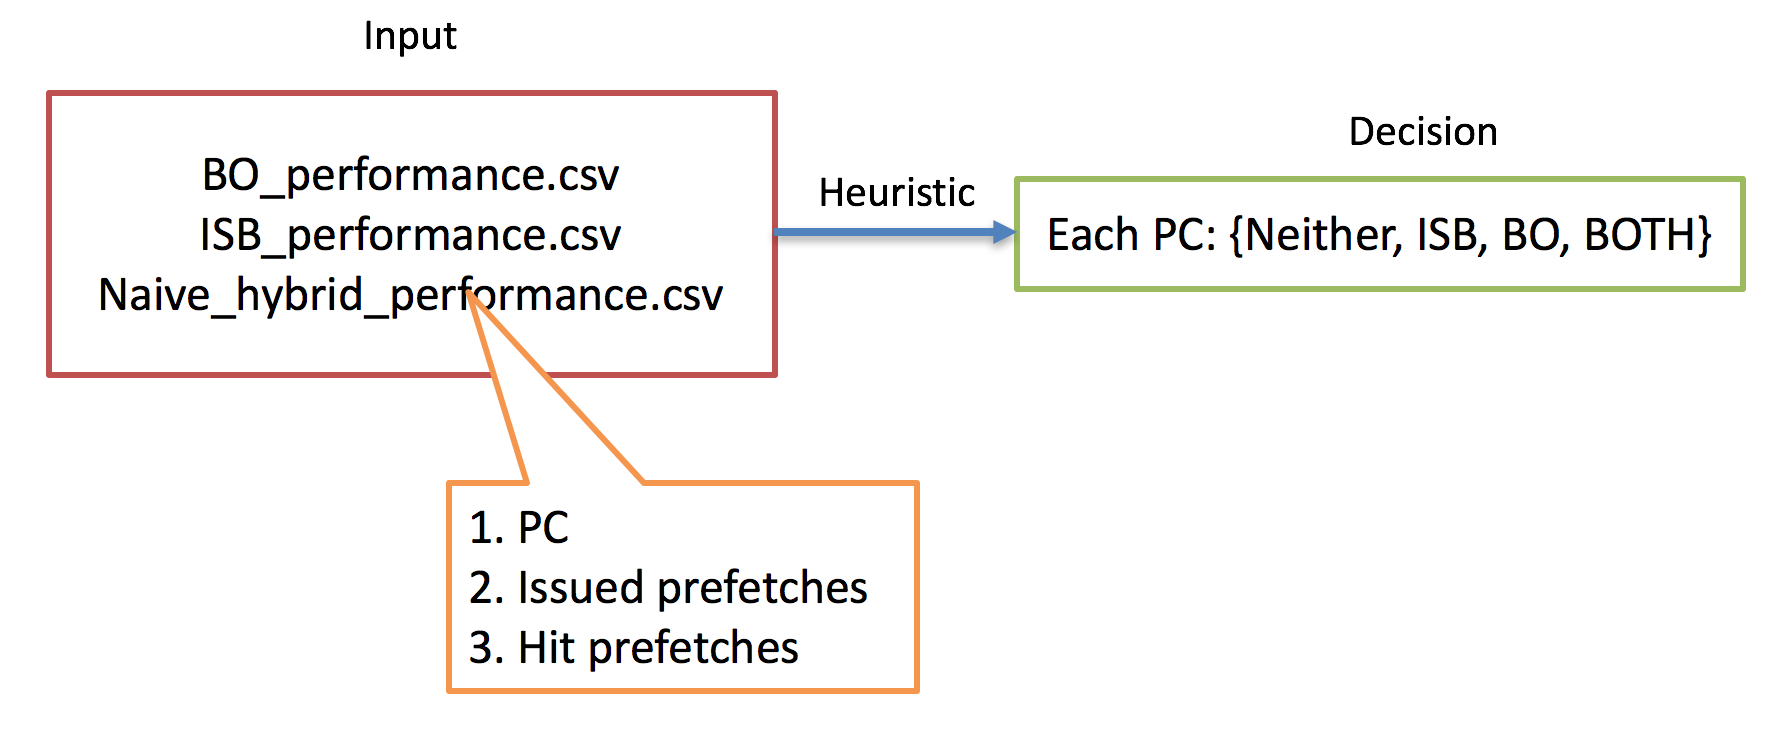
\includegraphics[width=0.8\textwidth]{images/staticanalysis_flow.png}
	  \caption{Static Analysis Design Flow}
	  \label{fig:staticanalysis_flow}
  \end{figure}


  \begin{figure}[ht!]
	  \centering
	  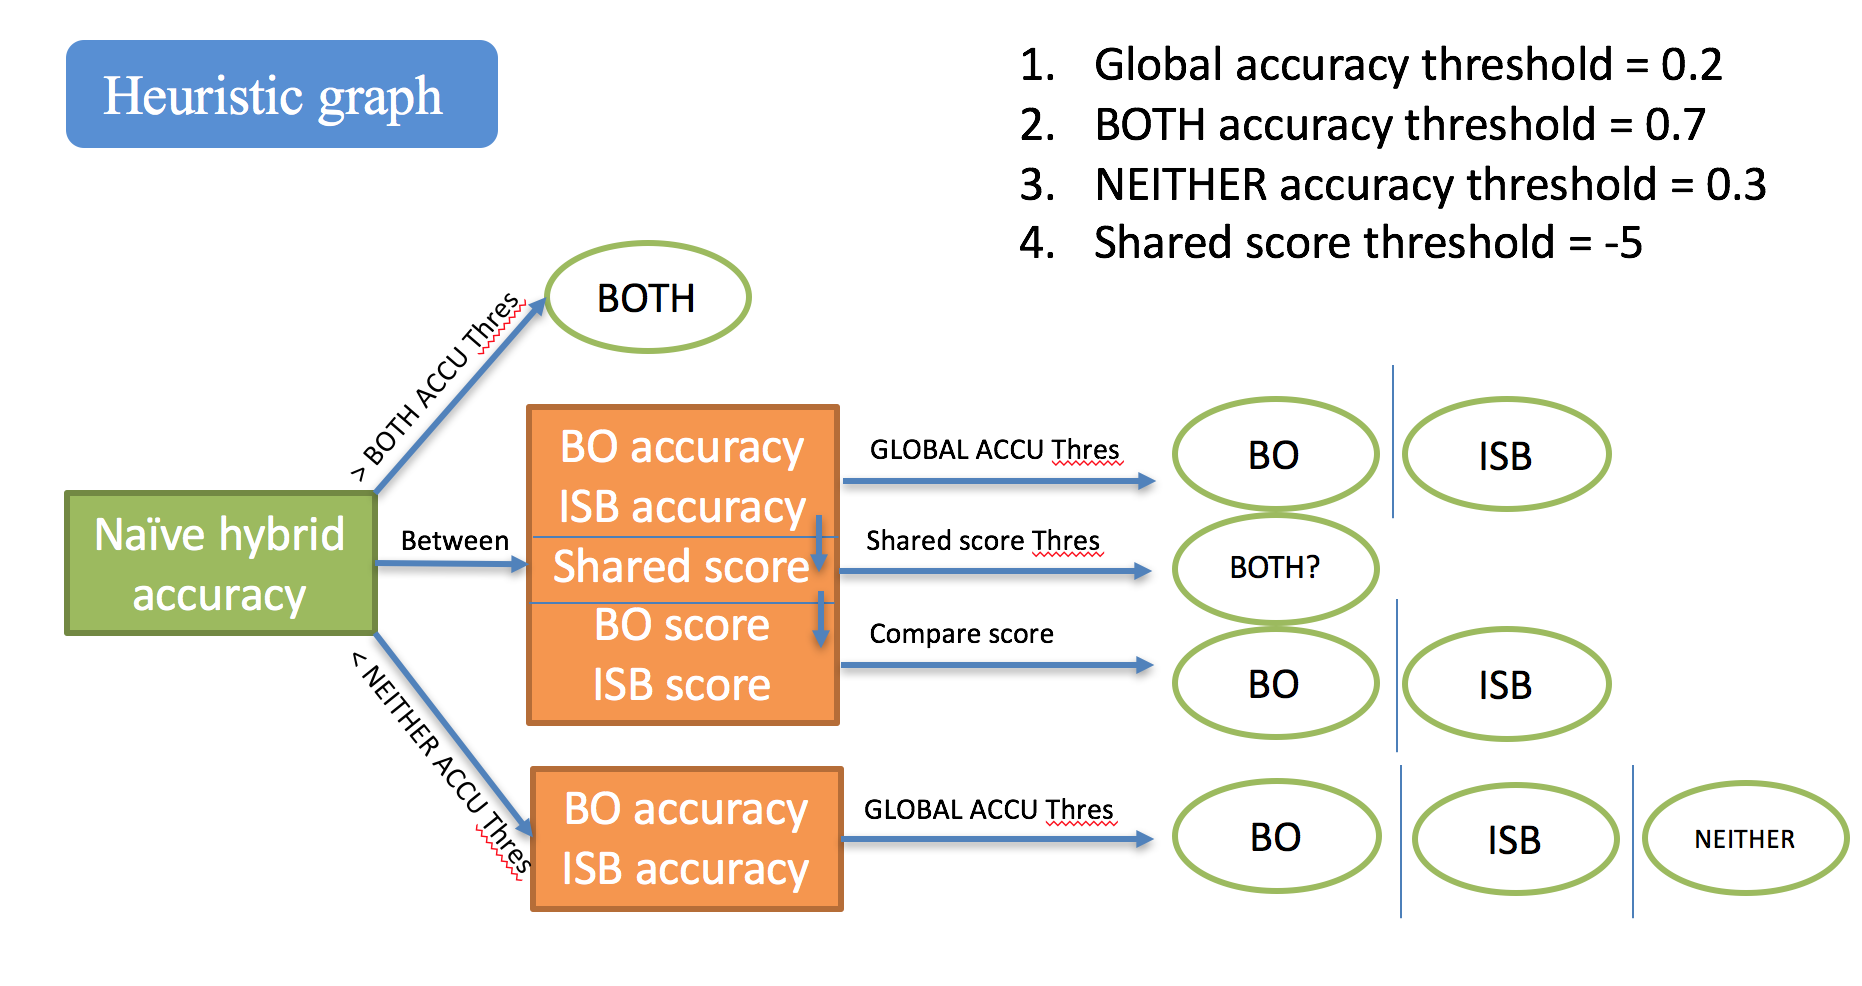
\includegraphics[width=0.8\textwidth]{images/heuristic_design.png}
	  \caption{Heuristic Design}
	  \label{fig:heuritic design}
  \end{figure}

  Here we will describle how our heuristic are designed in Fig.\ref{fig:heuritic design}. Four threshold are defined by user. \emph{Global Accuracy Threshold} set the lowest acceptable accuracy of one PC of any kind of prefetcher. \emph{BOTH Accuracy Threshold} determines when we should prefetch both. \emph{NEITHER Accuracy Threshold} determines when we should prefetch at most one of them. Last but not least, \emph{Shared Score Threshold} determines how should shared hits and shared prefetch affect the final decision. The decision process is list as follows.

  1) Compare \emph{NHP}'s accuracy with \emph{BOTH Accuracy Threshold}. If \emph{NHP}'s accuracy is higher than threshold, the hybrid prefetcher would choose both prefetches from \emph{ISB} and \emph{BO}.

  2) Compare \emph{NHP}'s accuracy with \emph{NEITHER Accuracy Threshold}. If \emph{NHP}'s accuracy is lower than threshold, the hybrid prefetcher would choose prefetches from either \emph{ISB}, or \emph{BO} or neither of them.

  3) Compare \emph{ISB}'s and \emph{BO}'s with \emph{Global Accuracy Threshold}, make decision when one meet the threshold and the the other does not. If both meet, go to step 4.

  4) Calculte the shared score. The shared score calculate how many shared hits and shared miss prefetch are made. Usually less share hits and more shared prefetches indicate better cache performance. The score is compared to \emph{Shared Score Threshold} in order to decide whether prefetch both or go to step 5. The score is calculated in equation.\ref{equ:shared_score}.

  \begin{equation}
  \label{equ:shared_score}
  shared\_score = shared\_hits - accuracy\_NHP * shared\_prefetch
  \end{equation}

  5) \emph{BO} score and \emph{ISB} score are defined in equation.\ref{equ:prefetcher_score}. The heuristic of this equation is to calulate the importance of hit and useless prefetches. Hits are more evaluated so we apply a coefficient to reduce the impact of useless prefetches. Finally, the hybrid prefetcher will pick the one with higher score.
  \begin{equation}
  \label{equ:prefetcher_score}
  score = hits - useless\_prefetch * (1 - accuracy\_NHP)
  \end{equation}
